%%%%%%%%%%%%%%%%%%%%%%%%%%%%%%%%%%%%%%%%%%%%%%%%%%%%%%%%%%%%%%%%%%%%%%%%%%%%%%%%%%%%%%%%%%%%%%%%%%%

%% document class
%\documentclass{beamer}
\documentclass[aspectratio=169]{beamer}
%\documentclass[handout]{beamer}

%% packages
\usepackage{multimedia}
\usepackage{tikz,lipsum,lmodern}
\usepackage[most]{tcolorbox}


%% page settings
%% Theme
%\usetheme{Berkeley} % theme for slides
\usetheme{AnnArbor}
%\usetheme{Frankfurt}
%\usetheme{Madrid}
%\usetheme{default}
%\usetheme{Goettingen}

%% Colors
\usecolortheme{seahorse} % color for slides
%\usecolortheme{default}
%\setbeamercolor{titlelike}{parent=structure,bg=green}

%%\setbeamercolor*{titlelike}{parent=palette primary}
\setbeamercolor{titlelike}{parent=palette primary,fg=black, bg=c3} %gray!30!white
\setbeamercolor{frametitle}{fg=black, bg=c1}
%\setbeamercolor{framesubtitle}{c3}
\setbeamercolor{frametitle right}{bg=gray!30!white}
%\definecolor{darkgray}{rgb}{gray!30!white}
\definecolor{c1}{rgb}{0,0.5,0.0} % some gray
\definecolor{c2}{rgb}{0.4,0.69,0.2} % some gray
\definecolor{c3}{rgb}{0.05,0.6,0.1} % some gray
%% see http://www.sharelatex.com/learn/Beamer
\setbeamercolor*{palette primary}{fg=white,bg=c3} % upper part
\setbeamercolor*{palette secondary}{bg=c3} % left part (background)
\setbeamercolor*{sidebar left}{fg=black,bg=c1} % left part with links
\setbeamerfont{section number projected}{ % section numbers
  family=\rmfamily,
  series=\bfseries,
  size=\normalsize
  }


\setbeamercolor{section number projected}{bg=c1} % color of section numbers and others (fg: Fontm, bg:Hintergrund)
\setbeamercolor{item projected}{bg=c1}
\setbeamercolor{itemize item}{fg=c1}
\setbeamercolor{author in sidebar}{fg=black}


%% Fonts
\usefonttheme{professionalfonts} % changes fonts

%% Foot
\usenavigationsymbolstemplate{} % deafult controls off
\setbeamertemplate{footline}[frame number] % slide number at the bottom
\setbeamertemplate{footline}
{%
\setbeamercolor{footlinecolor}{fg=black,bg=c3}
	\leavevmode%
	\hbox{%
	\begin{beamercolorbox}[wd=.3\paperwidth,ht=3ex,dp=1.5ex,left,leftskip=2mm]{footlinecolor}%
		www.bluehende-Heimat.de
	\end{beamercolorbox}%
	\begin{beamercolorbox}[wd=.5\paperwidth,ht=3ex,dp=1.5ex,left,leftskip=2mm]{footlinecolor}%
		manfred.kraft@bluehende-heimat.de
	\end{beamercolorbox}%
	\begin{beamercolorbox}[wd=.2\paperwidth,ht=3ex,dp=1.5ex,right,rightskip=2mm]{footlinecolor}%
		\insertframenumber{} / \inserttotalframenumber%
	\end{beamercolorbox}%
	}%
	\vskip0pt%
}

%% new commands
\newcommand{\cm}[1]{{\tt \textcolor{white}{#1}}}
\newcommand{\wl}[2]{\href{#2}{\textcolor{blue}{#1}}}
\newcommand{\att}[2]{\href{#2}{\textcolor{blue}{#1}}}


\useoutertheme{infolines}

%\logo { 
%\begin{tikzpicture}[overlay,remember picture]
%\node[right=0.06cm] at (current page.148){
%    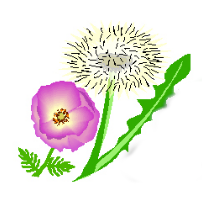
\includegraphics[width=1.3cm]{figures/BH-Logo_Quat.png}
%};
%\end{tikzpicture}
%}

%%%%%%%%%%%%%%%%%%%%%%%%%%%%%%%%%%%%%%%%%%%%%%%%%%%%%%%%%%%%%%%%%%%%%%%%%%%%%%%%%%%%%%%%%%%%%%%%%%%
%%%%%%%%%%%%%%%%%%%%%%%%%%%%%%%%%%%%%%%%%%%%%%%%%%%%%%%%%%%%%%%%%%%%%%%%%%%%%%%%%%%%%%%%%%%%%%%%%%%

\begin{document}

%%%%%%%%%%%%%%%%%%%%%%%%%%%%%%%%%%%%%%%%%%%%%%%%%%%%%%%%%%%%%%%%%%%%%%%%%%%%%%%%%%%%%%%%%%%%%%%%%%%
%%%%%%%%%%%%%%%%%%%%%%%%%%%%%%%%%%%%%%%%%%%%%%%%%%%%%%%%%%%%%%%%%%%%%%%%%%%%%%%%%%%%%%%%%%%%%%%%%%%
%%%%%%%%%%%%%%%%%%%%%%%%%%%%%%%%%%%%%%%%%%%%%%%%%%%%%%%%%%%%%%%%%%%%%%%%%%%%%%%%%%%%%%%%%%%%%%%%%%%

\author[Manfred]{Manfred Kraft}
 
\title[Vespa velutina-240310]{\textbf{Asiatische Hornisse \\ Vespa velutina nigrithorax}}
\titlegraphic{
\includegraphics[width=0.40\textwidth]{figures/BH-Logo.png}}
\institute{www.bluehende-Heimat.de}
\date{Unterkirnach, \today}

\frame{\titlepage}


%%%%%%%%%%%%%%%%%%%%%%%%%%%%%%%%%%%%%%%%%%%%%%%%%%%%%%%%%%%%%%%%%%%%%%%%%%%%%%%%%%%%%%%%%%%%%%%%%%%
%%%%%%%%%%%%%%%%%%%%%%%%%%%%%%%%%%%%%%%%%%%%%%%%%%%%%%%%%%%%%%%%%%%%%%%%%%%%%%%%%%%%%%%%%%%%%%%%%%%

\begin{frame}{Ausgangs-Situation}
\frametitle{{Vespa velutina, eine invasive Art}}
\framesubtitle{\cm{Lebensweise und Lebensraum}} 


%\tableofcontents
\tableofcontents[hideallsubsections]
\end{frame}                 

%%%%%%%%%%%%%%%%%%%%%%%%%%%%%%%%%%%%%%%%%%%%%%%%%%%%%%%%%%%%%%%%%%%%%%%%%%%%%%%%%%%%%%%%%%%%%%%%%%%
\section{Herkunft}

\subsection[Ausgangslage]{Herkunft der Vespa velutina}

\subsubsection[Ursprung]{Ursprung}

\begin{frame}{Herkunft der Vespa velutina}
	\framesubtitle{\cm{Wo ist die Vespa velutina ursprünglich beheimatet?}} 

	\begin{examples}{Reproduktionsphase:  }{bis 250 Jungköniginnen!}
		\begin{center}	
			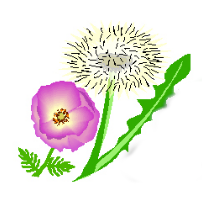
\includegraphics[width=0.2\textwidth]{figures/BH-Logo_Quat.png}
		\end{center}
		\end{examples}
%\tableofcontents[currentsection,hidesubsections]
\end{frame}

\subsubsection[Ankunft in Europa]{Ankunft in Europa}

\begin{frame}{Ankunft in Europa}
	%\framesubtitle{\cm{Herkunft der Vespa velutina}}

	\begin{examples}{Reproduktionsphase:  }{bis 250 Jungköniginnen!}
		\begin{center}	
			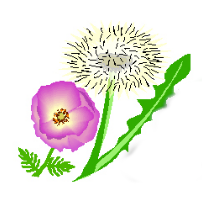
\includegraphics[width=0.2\textwidth]{figures/BH-Logo_Quat.png}
		\end{center}
		\end{examples}
%\tableofcontents[currentsection,hidesubsections]
\end{frame}

\subsubsection[Ankunft in Deutschland]{Ankunft in Deutschland}

\begin{frame}{Ankunft in Deutschland}
	%\framesubtitle{\cm{Herkunft der Vespa velutina}}

	\begin{examples}{Reproduktionsphase:  }{bis 250 Jungköniginnen!}
		\begin{center}	
			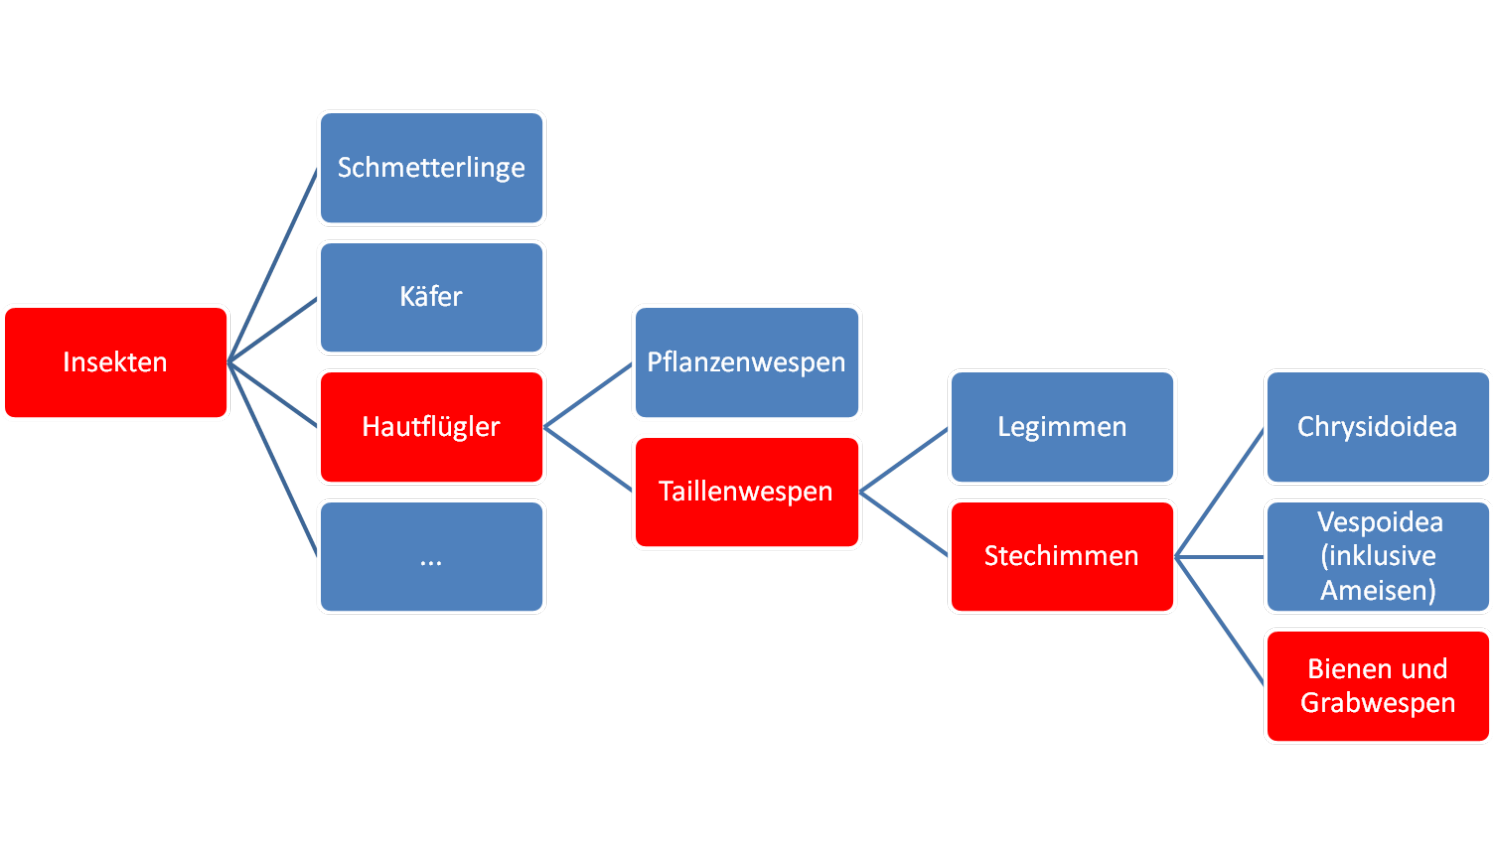
\includegraphics[width=0.6\textwidth]{figures/Insekten-31.png}
		\end{center}
		\end{examples}
%\tableofcontents[currentsection,hidesubsections]
\end{frame}

%%%%%%%%%%%%%%%%%%%%%%%%%%%%%%%%%%%%%%%%%%%%%%%%%%%%%%%%%%%%%%%%%%%%%%%%%%%%%%%%%%%%%%%%%%%%%%%%%%%
\section{Lebensweise und Lebensraum der Vespa velutina}

\subsection{Aussehen und Lebensweise}

%%%%%%%%%%%%%%%%%%%%%%%%%%%%%%%%%%%%%%%%%%%%%%%%%%%%%%%%%%%%%%%%%%%%%%%%%%%%%%%%%%%%%%%%%%%%%%%%%%%%

\subsubsection[Allgemeine Information]{Allgemeine Information}

\begin{frame}{Allgemeine Information}
	\framesubtitle{\cm{Aussehen und Lebensweise}} 

\begin{examples}{Reproduktionsphase:  }{bis 250 Jungköniginnen!}
		\begin{center}	
			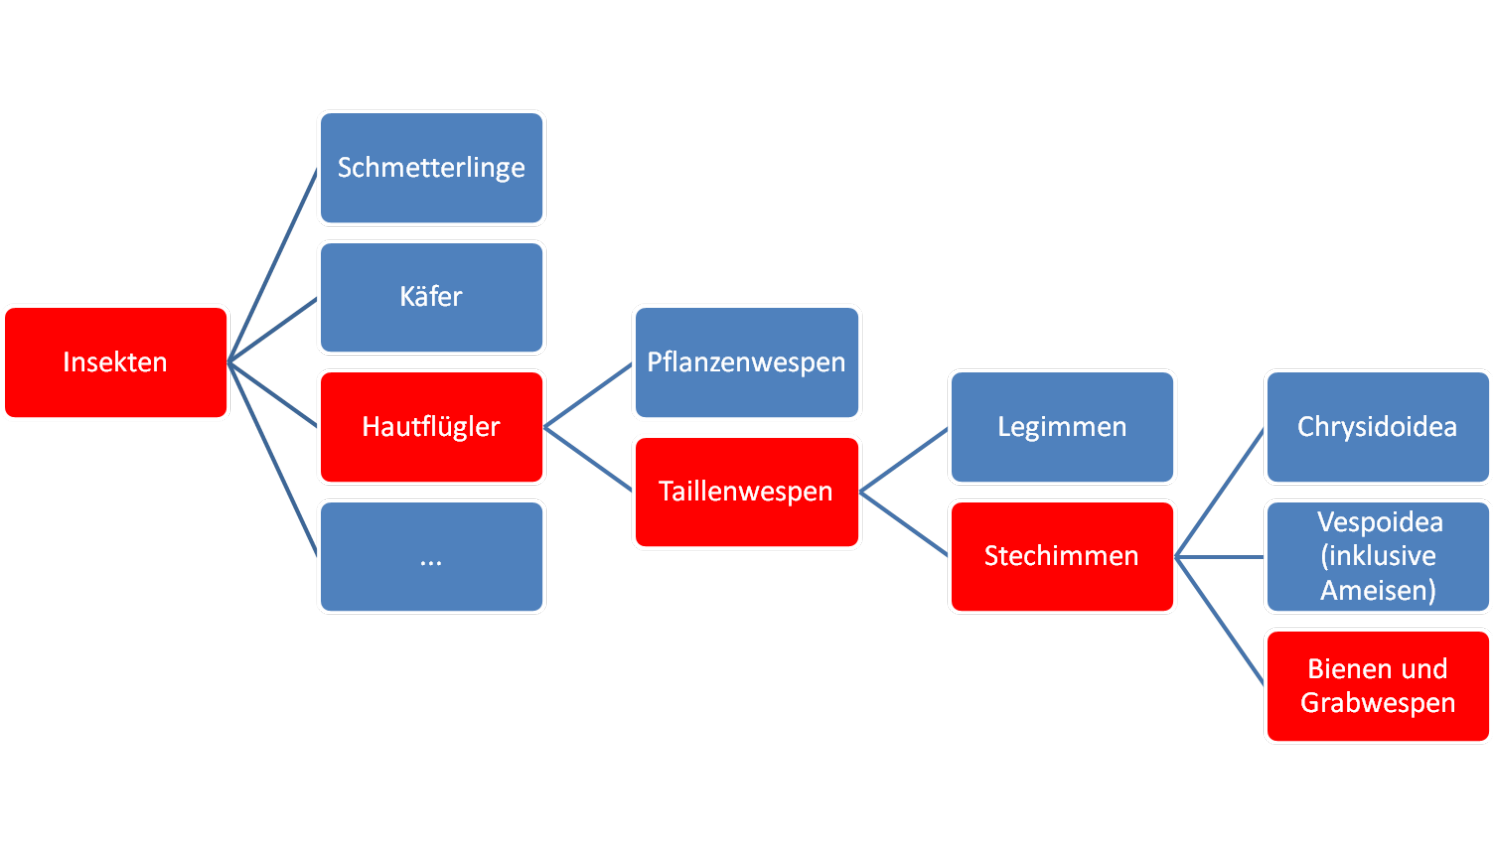
\includegraphics[width=0.2\textwidth]{figures/Insekten-31.png}
		\end{center}
		\end{examples}

	\end{frame}

\subsubsection[Körperbau]{Körperbau}

\begin{frame}{Aussehen und Verhalten}
	\framesubtitle{\cm{Aussehen und Lebensweise}} 
	\begin{center}	
		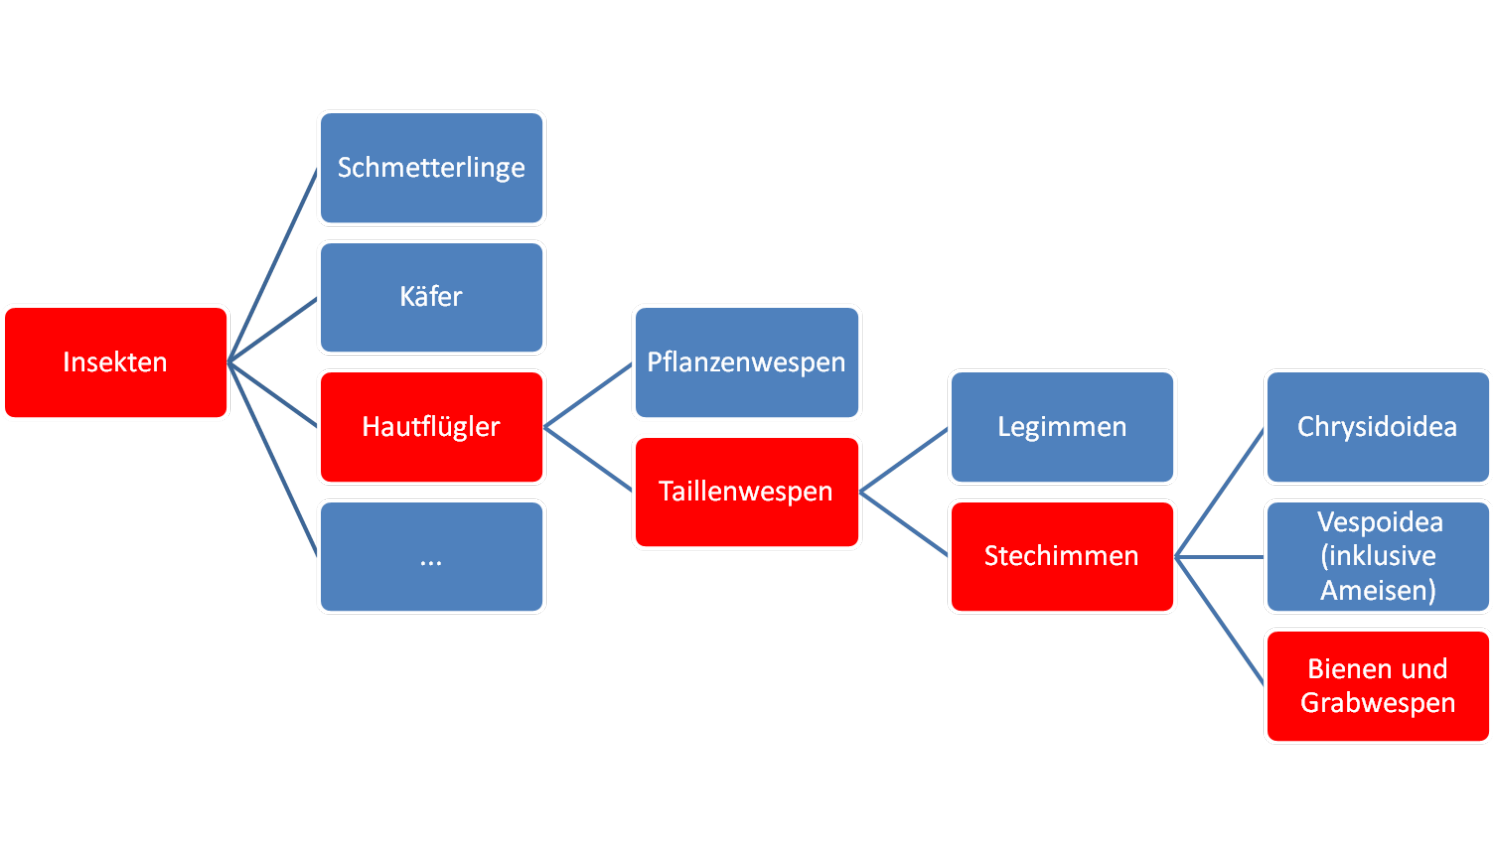
\includegraphics[width=0.8\textwidth]{figures/Insekten-31.png}
	\end{center}
\end{frame}

\begin{frame}{Unterschiede Männliches und weibliches Insekt}
	\framesubtitle{\cm{Aussehen und Lebensweise}} 

	\begin{center}	
		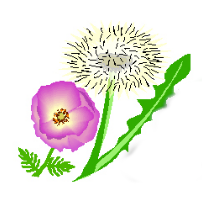
\includegraphics[width=0.2\textwidth]{figures/BH-Logo_Quat.png}
	\end{center}

	\end{frame}

\subsubsection[Verwechslungsgefahr]{Verwechslungsgefahr mit der europ. Hornisse}

\begin{frame}{Verwechslungsgefahr mit der europ. Hornisse 1}
	\framesubtitle{\cm{Aussehen und Lebensweise}} 
	\begin{center}	
		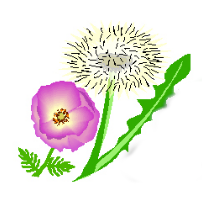
\includegraphics[width=0.2\textwidth]{figures/BH-Logo_Quat.png}
	\end{center}
	\end{frame}



%%%%%%%%%%%%%%%%%%%%%%%%%%%%%%%%%%%%%%%%%%%%%%%%%%%%%%%%%%%%%%%%%%%%%%%%%%%%%%%%%%%%%%%%%%%%%%%%%%%%

\subsection[Entwicklung]{Entwicklung der Hornisse}

\begin{frame}{Entwicklung der Vespa velutina}

	\begin{center}	
		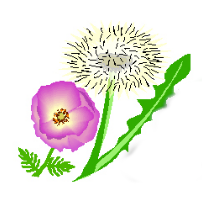
\includegraphics[width=0.2\textwidth]{figures/BH-Logo_Quat.png}
	\end{center}

	\end{frame}

	\begin{frame}{Wabe der Vespa velutina}
		\begin{center}	
			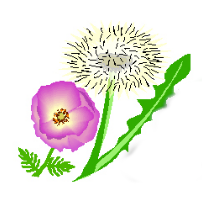
\includegraphics[width=0.2\textwidth]{figures/BH-Logo_Quat.png}
		\end{center}

		\end{frame}

%%%%%%%%%%%%%%%%%%%%%%%%%%%%%%%%%%%%%%%%%%%%%%%%%%%%%%%%%%%%%%%%%%%%%%%%%%%%%%%%%%%%%%%%%%%%%%%%%%%%

\subsection[Nester]{Nester der Vespa velutina}

\begin{frame}{Nester der Vespa velutina}
    \frametitle{Nester der Vespa velutina} 
    \framesubtitle{Die verschiedenen Nester der Hornisse}
    \begin{itemize} 
        \item 
            Embryonal-Nester \pause
        \item 
            Primär-Nest \pause
        \item 
            Sekundärnest 
    \end{itemize}
 
    \end{frame}

\subsubsection[Embryonal-Nest]{Embryonal-Nest}


	\begin{frame}{Embryonal-Nest}
		\begin{center}	
			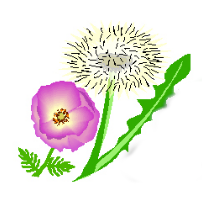
\includegraphics[width=0.2\textwidth]{figures/BH-Logo_Quat.png}
		\end{center}

		\end{frame}

\subsubsection[Sekundär-Nest]{Primär-Nest}


		\begin{frame}{Primär-Nest}
			\begin{center}	
				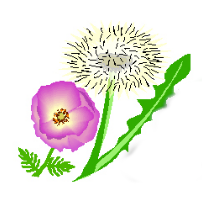
\includegraphics[width=0.2\textwidth]{figures/BH-Logo_Quat.png}
			\end{center}
	
			\end{frame}

\subsubsection[Sekundär-Nest]{Sekundär-Nest}


			\begin{frame}{Sekundär-Nest}
				\begin{center}	
					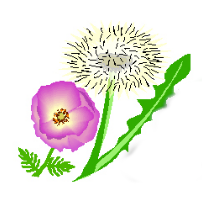
\includegraphics[width=0.2\textwidth]{figures/BH-Logo_Quat.png}
				\end{center}
		
				\end{frame}


\subsubsection[Reproduktionsphase]{Reproduktionsphase}

\begin{frame}{Reproduktionsphase}
\frametitle{Reproduktionsphase} 
\framesubtitle{Wie vermehrt sich die Vespa velutina?}

\begin{examples}{Reproduktionsphase:  }{bis 250 Jungköniginnen!}
\begin{center}	
    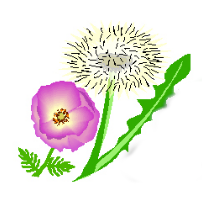
\includegraphics[width=0.2\textwidth]{figures/BH-Logo_Quat.png}
\end{center}
\end{examples}
\end{frame}

\subsubsection{Lebenszyklus der Vespa velutina}
%%%%%%%%%%%%%%%%%%%%%%%%%%%%%%%%%%%%%%%%%%%%%%%%%%%%%%%%%%%%%%%%%%%%%%%%%%%%%%%%%%%%%%%%%%%%%%%%
%%%%%%%%%%%%%%%%%%%%%%%%%%%%%%%%%%%%%%%%%%%%%%%%%%%%%%%%%%%%%%%%%%%%%%%%%%%%%%%%%%%%%%%%%%%%%%%%%%%
\section{Auswirkungen auf die Biodiversität und die Menschen}
%%%%%%%%%%%%%%%%%%%%%%%%%%%%%%%%%%%%%%%%%%%%%%%%%%%%%%%%%%%%%%%%%%%%%%%%%%%%%%%%%%%%%%%%%%%%%%%%
%%%%%%%%%%%%%%%%%%%%%%%%%%%%%%%%%%%%%%%%%%%%%%%%%%%%%%%%%%%%%%%%%%%%%%%%%%%%%%%%%%%%%%%%%%%%%%%%%%%
\section{Bekämpfung der vespa velutina}
%%%%%%%%%%%%%%%%%%%%%%%%%%%%%%%%%%%%%%%%%%%%%%%%%%%%%%%%%%%%%%%%%%%%%%%%%%%%%%%%%%%%%%%%%%%%%%%%
%%%%%%%%%%%%%%%%%%%%%%%%%%%%%%%%%%%%%%%%%%%%%%%%%%%%%%%%%%%%%%%%%%%%%%%%%%%%%%%%%%%%%%%%%%%%%%%%%%%
%\section{Auswirkungen}
%%%%%%%%%%%%%%%%%%%%%%%%%%%%%%%%%%%%%%%%%%%%%%%%%%%%%%%%%%%%%%%%%%%%%%%%%%%%%%%%%%%%%%%%%%%%%%%%
%%%%%%%%%%%%%%%%%%%%%%%%%%%%%%%%%%%%%%%%%%%%%%%%%%%%%%%%%%%%%%%%%%%%%%%%%%%%%%%%%%%%%%%%%%%%%%%%%%%




%%%%????????????????????????????????????????????????????????????????%%%%%%%%%%%%%%%%%%%%%%%%%%%%%

\begin{frame}{Gruppenarbeit}
	\frametitle{Wie können wir unsere Ziele erreichen?} 
	\framesubtitle{... durch Gruppenarbeit.}
\tableofcontents[currentsection,hidesubsections]
\end{frame}
%%%%%%%%%%%%%%%%%%%%%%%%%%%%%%%%%%%%%%%%%%%%%%%%%%%%%%%%%%%%%%%%%%%%%%%%%%%%%%%%%%%%%%%%%%%%%%%%%%%
%%%%%%%%%%%%%%%%%%%%%%%%%%%%%%%%%%%%%%%%%%%%%%%%%%%%%%%%%%%%%%%%%%%%%%%%%%%%%%%%%%%%%%%%%%%%%%%%%%%
\subsection[Flächen]{Welche Flächen stehen uns zur Verfügung?}

\begin{frame}{Flächeneinteilung}
	\frametitle{In welcher Gruppe möchten Sie sich engagieren?} 
	\framesubtitle{Flächeneinteilung}

	\textbf{Flächeneinteilung}\\
	Wir haben die in Frage kommenden Flächen in drei Gruppen aufgeteilt:
	
	\begin{columns}[t]
	\column{0.45\textwidth}
		Flächen-Einteilung \\
		\visible<2->{
		\begin{enumerate}
		\item	
			Gärten \& Balkone
		\visible<3->{
		\item
			Straßen, Gehwege und Verkehrsinseln
		\visible<4>{
		\item
			Private und öffentliche Flächen
		%\visible<4>{
		%\item
		%	Point 4
		%}
		}
		\end{enumerate}	
		}}
	\column{0.5\textwidth}
		\mbox{} \\
		\begin{overlayarea}{\textwidth}{0.4\textheight}
		\only<2>{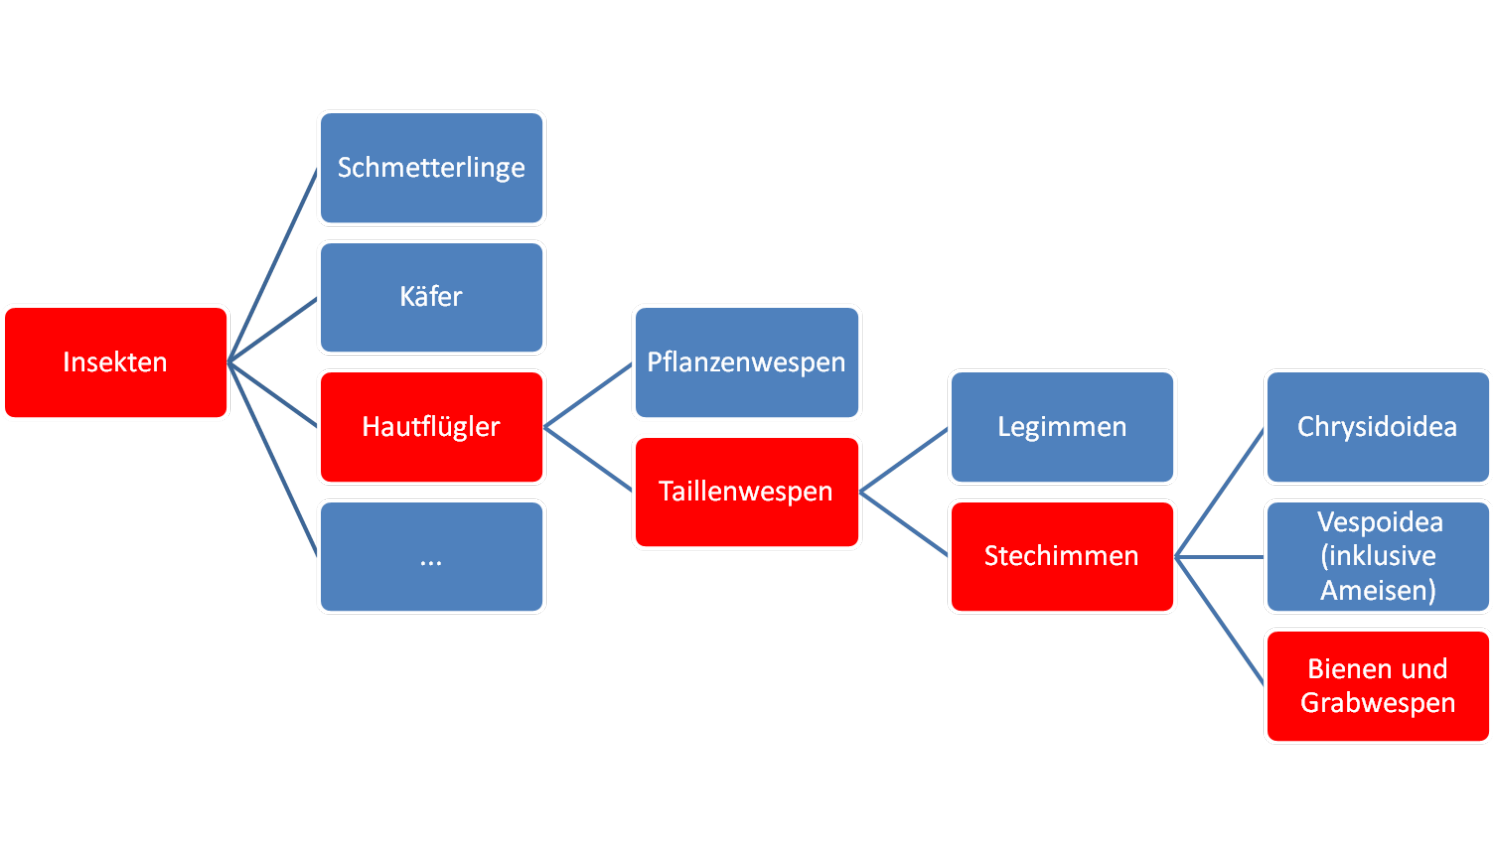
\includegraphics[width=0.6\textwidth]{figures/Insekten-31.png}}

		\only<3>{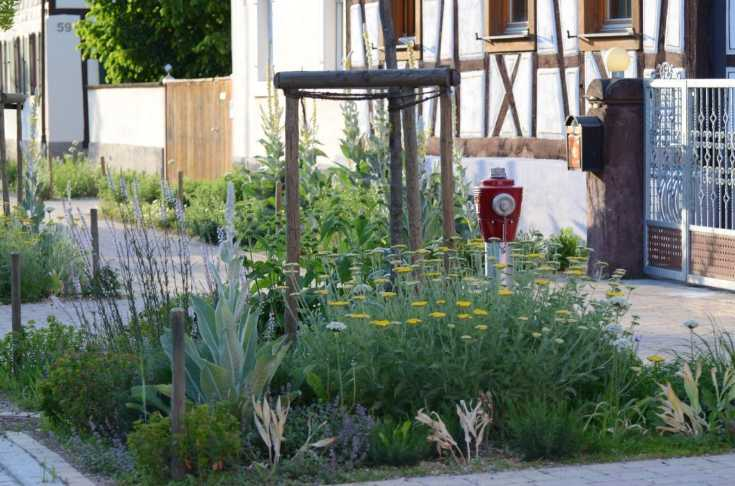
\includegraphics[width=0.8\textwidth]{figures/Strasse.jpg}}
		\only<4>{\includegraphics[width=0.8\textwidth]{figures/Blühwiese.jpg}}
		\end{overlayarea}
		%
	\end{columns}
	
	\end{frame}

%%%%%%%%%%%%%%%%%%%%%%%%%%%%%%%%%%%%%%%%%%%%%%%%%%%%%%%%%%%%%%%%%%%%%%%%%%%%%%%%%%%%%%%%%%%%%%%%%%%
\subsection{Gruppen-Arbeit}

\begin{frame}{Gruppen-Einteilung}
	\frametitle{In welcher Gruppe möchten Sie sich engagieren?} 
	\framesubtitle{Gruppen-Einteilung}

	\textbf{Gruppen-Einteilung}\\
	Wir haben die in Frage kommenden Flächen in drei Gruppen aufgeteilt:\\
	Merken Sie sich bitte Ihre Gruppe:
	\begin{columns}[t]
	\column{0.45\textwidth}
		\\
		\visible<2->{
		\begin{enumerate}
		\item	
		\textbf{Gruppe "Garten" }: Gärten \& Balkone
		\visible<3->{
		\item
			Gruppe \textbf{"Strasse" }: Straßen, Gehwege und Verkehrsinseln
			\visible<4->{
		\item
			Gruppe \textbf{"Blühfläche" }: Private und öffentliche Flächen
		\visible<5>{
		\item
			Gruppe \textbf{"Öffentlichkeitsarbeit" }:
		}
		}}
		\end{enumerate}	
		}
	\column{0.5\textwidth}
		\mbox{} \\
		\begin{overlayarea}{\textwidth}{0.4\textheight}
		\only<2->{\includegraphics[width=0.35\textwidth]{figures/Vorgarten.jpg}}
		\only<3->{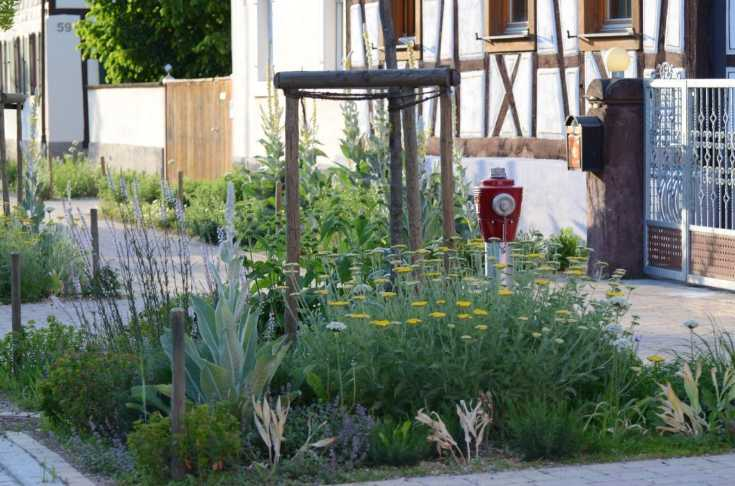
\includegraphics[width=0.35\textwidth]{figures/Strasse.jpg}}
		\only<4->{\includegraphics[width=0.35\textwidth]{figures/Blühwiese.jpg}}
		\end{overlayarea}

	\end{columns}	
\end{frame}

%%%%%%%%%%%%%%%%%%%%%%%%%%%%%%%%%%%%%%%%%%%%%%%%%%%%%%%%%%%%%%%%%%%%%%%%%%%%%%%%%%%%%%%%%%%%%%%%%%%
%%%%%%%%%%%%%%%%%%%%%%%%%%%%%%%%%%%%%%%%%%%%%%%%%%%%%%%%%%%%%%%%%%%%%%%%%%%%%%%%%%%%%%%%%%%%%%%%%%%

\section{Lebensraum der Vespa velutina}

%%%%%%%%%%%%%%%%%%%%%%%%%%%%%%%%%%%%%%%%%%%%%%%%%%%%%%%%%%%%%%%%%%%%%%%%%%%%%%%%%%%%%%%%%%%%%%%%%%%%

\begin{frame}{Gruppenarbeit}
\frametitle{Zusammenfassung} 
\framesubtitle{Vorstellung der Gruppenergebnisse.}
\tableofcontents[currentsection,hidesubsections]
\end{frame}
%%%%%%%%%%%%%%%%%%%%%%%%%%%%%%%%%%%%%%%%%%%%%%%%%%%%%%%%%%%%%%%%%%%%%%%%%%%%%%%%%%%%%%%%%%%%%%%%%%%
%%%%%%%%%%%%%%%%%%%%%%%%%%%%%%%%%%%%%%%%%%%%%%%%%%%%%%%%%%%%%%%%%%%%%%%%%%%%%%%%%%%%%%%%%%%%%%%%%%%
\subsection[Garten]{Summary Gruppe "Garten"}


\begin{frame}{Garten}
	\frametitle{Zusammenfassung Gruppe "Garten"} 
	\framesubtitle{Vorstellung der Gruppenergebnisse.}
	Zusammenfassung Gruppe "Garten"
\end{frame}

%%%%%%%%%%%%%%%%%%%%%%%%%%%%%%%%%%%%%%%%%%%%%%%%%%%%%%%%%%%%%%%%%%%%%%%%%%%%%%%%%%%%%%%%%%%%%%%%%%%
\subsection[Strasse]{Summary Gruppe "Strasse"}

\begin{frame}{Strasse}
\frametitle{Zusammenfassung Gruppe "Strasse"} 
\framesubtitle{Vorstellung der Gruppenergebnisse}
Zusammenfassung Gruppe "Strasse"
\end{frame}

%%%%%%%%%%%%%%%%%%%%%%%%%%%%%%%%%%%%%%%%%%%%%%%%%%%%%%%%%%%%%%%%%%%%%%%%%%%%%%%%%%%%%%%%%%%%%%%%%%%
\subsection[Blühfläche]{Summary Gruppe "Blühfläche"}

\begin{frame}{Blühfläche}
\frametitle{Zusammenfassung Gruppe "Blühfläche"} 
\framesubtitle{Vorstellung der Gruppenergebnisse}
Zusammenfassung Gruppe "Blühfläche"
\end{frame}
%%%%%%%%%%%%%%%%%%%%%%%%%%%%%%%%%%%%%%%%%%%%%%%%%%%%%%%%%%%%%%%%%%%%%%%%%%%%%%%%%%%%%%%%%%%%%%%%%%%
%%%%%%%%%%%%%%%%%%%%%%%%%%%%%%%%%%%%%%%%%%%%%%%%%%%%%%%%%%%%%%%%%%%%%%%%%%%%%%%%%%%%%%%%%%%%%%%%%%%

\section[Heimische Insekten]{Verwechselungsgefahr!}

%%%%%%%%%%%%%%%%%%%%%%%%%%%%%%%%%%%%%%%%%%%%%%%%%%%%%%%%%%%%%%%%%%%%%%%%%%%%%%%%%%%%%%%%%%%%%%%%%%%%

\begin{frame}{Unterstützung}
\frametitle{Wo bekommen wir Unterstützung her?} 
\framesubtitle{Handel. Gewerbe \& Wettbewerbe}

\textbf{Sponsoren, Wettbewerbe etc.}\\
Finanzielle Unterstützung bei der Anlage und Betreuung der Blühflächen:

\begin{itemize}
	\item 
	\textbf{Handel \& Gewerbe} \pause 
	\item
	Wettbewerb \textbf{BWblüht} \pause
	\item 
	Wettbewerb \textbf{Burda} \pause
	\item 
	Wettbewerb \textbf{EDEKA}%\pause

\end{itemize}
\end{frame}



%%%%%%%%%%%%%%%%%%%%%%%%%%%%%%%%%%%%%%%%%%%%%%%%%%%%%%%%%%%%%%%%%%%%%%%%%%%%%%%%%%%%%%%%%%%%%%%%%%%
%%%%%%%%%%%%%%%%%%%%%%%%%%%%%%%%%%%%%%%%%%%%%%%%%%%%%%%%%%%%%%%%%%%%%%%%%%%%%%%%%%%%%%%%%%%%%%%%%%%

\section{Meldepflicht}

%%%%%%%%%%%%%%%%%%%%%%%%%%%%%%%%%%%%%%%%%%%%%%%%%%%%%%%%%%%%%%%%%%%%%%%%%%%%%%%%%%%%%%%%%%%%%%%%%%%%
\begin{frame}{Meldepflicht}
\frametitle{Meldepflicht} 
\framesubtitle{Vorschlag eines Projekt-Plans}
%\tableofcontents[currentsection,hidesubsections]

\begin{center}
	
	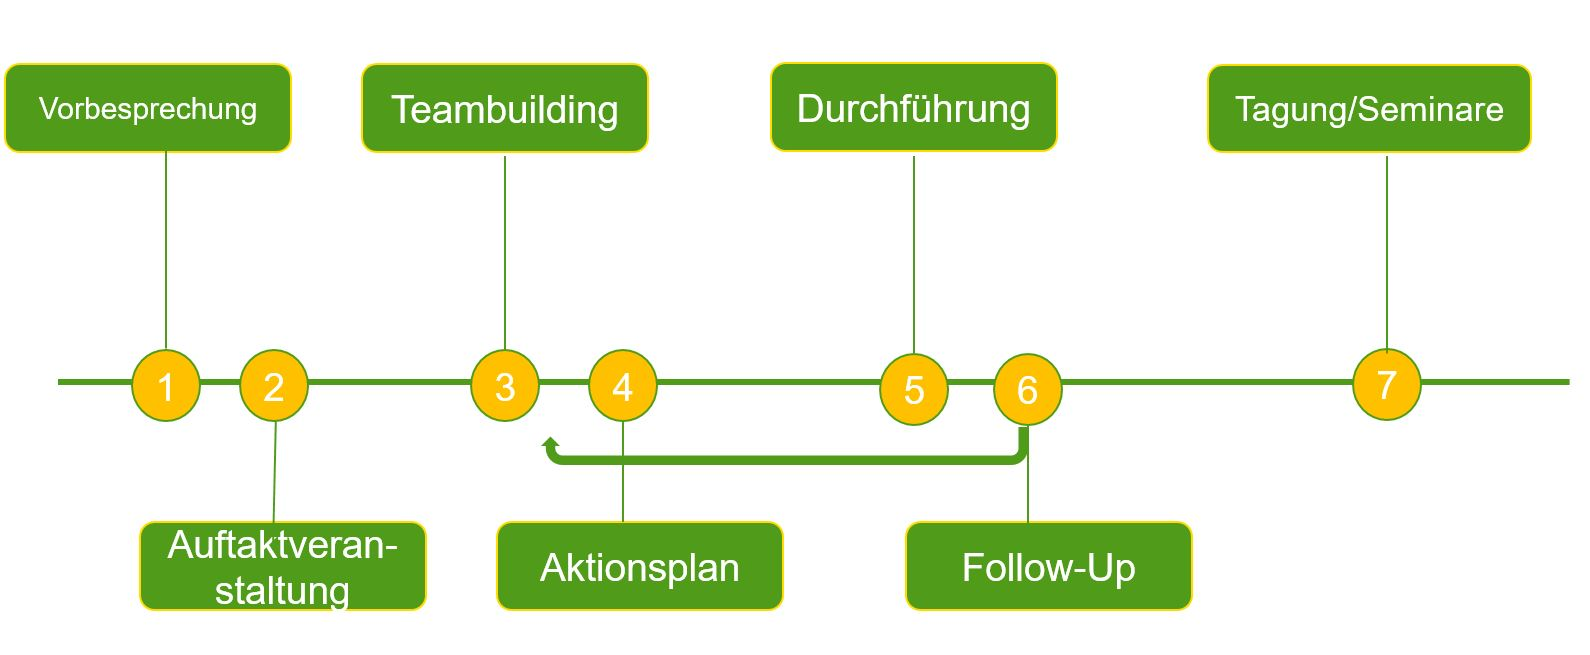
\includegraphics[width=1.0\textwidth]{figures/Ablaufschema.JPG}
	
\end{center}

\end{frame}
%%%%%%%%%%%%%%%%%%%%%%%%%%%%%%%%%%%%%%%%%%%%%%%%%%%%%%%%%%%%%%%%%%%%%%%%%%%%%%%%%%%%%%%%%%%%%%%%%%%
%%%%%%%%%%%%%%%%%%%%%%%%%%%%%%%%%%%%%%%%%%%%%%%%%%%%%%%%%%%%%%%%%%%%%%%%%%%%%%%%%%%%%%%%%%%%%%%%%%%
\subsection[Aufgaben]{Wie geht's weiter?}

\begin{frame}{Wie geht's weiter?}
	\frametitle{Anstehende Aufgaben} 
	\framesubtitle{Frühjahr 2024}

	\textbf{Nächste Schritte:}\\
	\begin{itemize}
		\item 
			Besichtigung der Flächen : 
			\textbf{Termin?} \pause 
		\item 
			Vorbereitung und Bewerbung : 
			\textbf{Wettbewerbe} \pause 
		\item 
			Saatgut bestellen \pause
		\item 
			Flächen vorbereiten \pause
		\item 
			Einsaat \pause
		\item 
			Nächste Schritte...%\pause
	\end{itemize}
	\begin{center}
	\textbf{Packen wir's an....}	
	\end{center}
\end{frame}

%%%%%%%%%%%%%%%%%%%%%%%%%%%%%%%%%%%%%%%%%%%%%%%%%%%%%%%%%%%%%%%%%%%%%%%%%%%%%%%%%%%%%%%%%%%%%%%%%%%
%%%%%%%%%%%%%%%%%%%%%%%%%%%%%%%%%%%%%%%%%%%%%%%%%%%%%%%%%%%%%%%%%%%%%%%%%%%%%%%%%%%%%%%%%%%%%%%%%%%

\section[Aufgaben]{Wie finden wir die Nester?}

%%%%%%%%%%%%%%%%%%%%%%%%%%%%%%%%%%%%%%%%%%%%%%%%%%%%%%%%%%%%%%%%%%%%%%%%%%%%%%%%%%%%%%%%%%%%%%%%%%%%
\begin{frame}{Wie geht's weiter?}
	\frametitle{Anstehende Aufgaben} 
	\framesubtitle{Frühjahr 2024}
	
	\textbf{Nächste Schritte:}\\
	\begin{itemize}
		\item 
		Besichtigung der Flächen : 
		\textbf{Termin?} \pause 
		\item 
		Vorbereitung und Bewerbung : 
		\textbf{Wettbewerbe} \pause 
		\item 
		Saatgut bestellen \pause
		\item 
		Flächen vorbereiten \pause
		\item 
		Einsaat \pause
		\item 
		Nächste Schritte...%\pause
	\end{itemize}
	\begin{center}
		\textbf{Packen wir's an....}	
	\end{center}
\end{frame}

%%%%%%%%%%%%%%%%%%%%%%%%%%%%%%%%%%%%%%%%%%%%%%%%%%%%%%%%%%%%%%%%%%%%%%%%%%%%%%%%%%%%%%%%%%%%%%%%%%%
%%%%%%%%%%%%%%%%%%%%%%%%%%%%%%%%%%%%%%%%%%%%%%%%%%%%%%%%%%%%%%%%%%%%%%%%%%%%%%%%%%%%%%%%%%%%%%%%%%%

\end{document}

%%%%%%%%%%%%%%%%%%%%%%%%%%%%%%%%%%%%%%%%%%%%%%%%%%%%%%%%%%%%%%%%%%%%%%%%%%%%%%%%%%%%%%%%%%%%%%%%%%%
%%%%%%%%%%%%%%%%%%%%%%%%%%%%%%%%%%%%%%%%%%%%%%%%%%%%%%%%%%%%%%%%%%%%%%%%%%%%%%%%%%%%%%%%%%%%%%%%%%%
%%%%%%%%%%%%%%%%%%%%%%%%%%%%%%%%%%%%%%%%%%%%%%%%%%%%%%%%%%%%%%%%%%%%%%%%%%%%%%%%%%%%%%%%%%%%%%%%%%%
